\section{Lecture 3 - Building Bridges}
\begin{itemize}
    \item Suppose we have a simple bridge over water:
    \begin{center}
        \begin{tikzpicture}[line cap=round,line join=round,>=triangle 45,x=1cm,y=1cm]
            
            \draw [fill=blue,opacity=0.3] (-3,1) rectangle (3,0);
            \draw [] (-5,2)-- (-3,2);
            \draw [] (-3,2)-- (-3,0);
            \draw [] (-3,0)-- (3,0);
            \draw [] (3,0)-- (3,2);
            \draw [] (3,2)-- (5,2);
            \draw [very thick] (-3.4,2.2)-- (3.4,2.2);
            \draw [very thick] (-2,2.2)-- (-2,0);
            \draw [very thick] (-1,0)-- (-1,2.2);
            \draw [very thick] (0,2.2)-- (0,0);
            \draw [very thick] (1,0)-- (1,2.2);
            \draw [very thick] (2,2.2)-- (2,0);
            \end{tikzpicture}
    \end{center}
    where the horizontal platform is known as the \textbf{beam} and the vertical supports are known as \textbf{posts} (which comes from the german word for tree)
    \item Disadvantages of this bridge is that it can easily break and become unusable in the event of a flood. This can be modified to become a \textbf{truss} bridge:
    \begin{center}
        \begin{tikzpicture}[line cap=round,line join=round,>=triangle 45,x=1cm,y=1cm]
            \draw [fill=blue,opacity=0.3] (-3,1) rectangle (3,0);
            \draw [] (-5,2.2)-- (-3,2.2);
            \draw [] (-3,2.2)-- (-3,0);
            \draw [] (-3,0)-- (3,0);
            \draw [] (3,0)-- (3,2.2);
            \draw [] (3,2.2)-- (5,2.2);
            \draw [very thick] (-3,2.2)-- (3,2.2);

            \foreach \x in {-3,-2,...,2}
            \draw [very thick] (\x ,2.2)-- (0.5+\x ,3.07);

            \foreach \x in {-3,-2,...,2}
            \draw [very thick] (\x+1,2.2)-- (0.5+\x ,3.07);

            \draw [very thick] (-2.5,3.07) -- (2.5,3.07);
            \end{tikzpicture}
    \end{center}
    However this type of bridge needs constant maintenance and none of the truss bridges the Romans have built lasted to today.
    \item One of the oldest bridges (est. 5000 BC) was built across a large pond, known as the ``Sweet Track.'' The bridge was built in an X-shape and people could walk on top:
    \begin{center}
        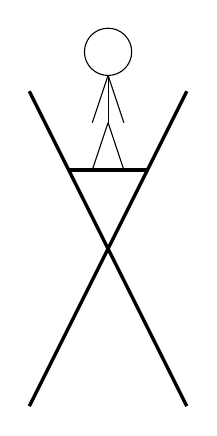
\begin{tikzpicture}
            \draw [very thick] (-1,2)-- (1,-2);
            \draw [very thick] (-1,-2)-- (1,2);
            \draw [] (0,2.2)-- (0,1.6);
            \draw [] (0,2.5) circle (0.3cm);
            \draw [very thick] (-0.5,1)-- (0.5,1);
            \draw [] (0,1.6)-- (-0.2,1);
            \draw [] (0,1.6)-- (0.2,1);
            \draw [] (0,2.2)-- (-0.2,1.6);
            \draw [] (0,2.2)-- (0.2,1.6);
        \end{tikzpicture}
    \end{center}
    \item Another form of bridge is suspended by hanging chains, known as a \textbf{suspension bridge}. A strong \textit{main cable} is pulled over two towers and fixed into concrete supports. Secondary \textit{hanging cables} run vertically and add support to the bridge.
    \begin{center}
        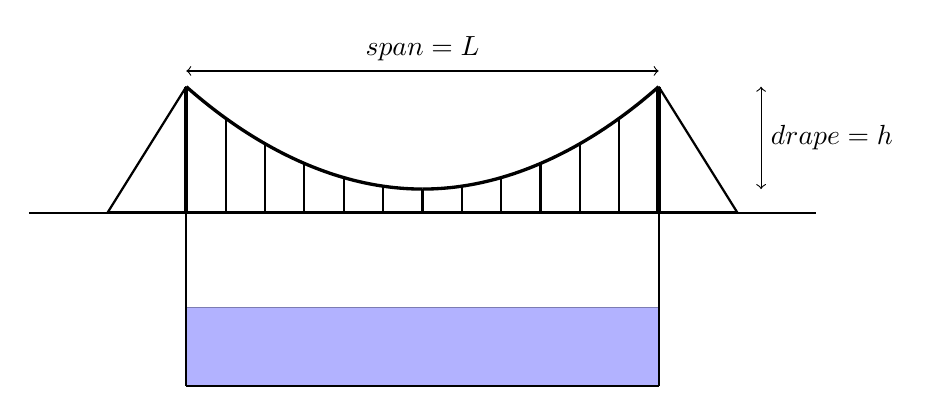
\begin{tikzpicture}
            \draw [fill=blue,opacity=0.3] (-3,1) rectangle (3,0);
            \draw [thick] (-5,2.2)-- (-3,2.2);
            \draw [thick] (-3,2.2)-- (-3,0);
            \draw [thick] (-3,0)-- (3,0);
            \draw [thick] (3,0)-- (3,2.2);
            \draw [thick] (3,2.2)-- (5,2.2);
            
            \draw [very thick] (0,2.5) parabola (3,3.8);
            \draw [very thick] (0,2.5) parabola (-3,3.8);
            \draw [very thick] (-4,2.2)-- (4,2.2);

            \foreach \x in {-2.5,-2,...,2.5}
            \draw [thick] (\x ,2.2)-- (\x ,0.144*\x*\x+2.5);

            \draw [ultra thick] (-3 ,2.2)-- (-3,3.8);
            \draw [thick] (-4,2.2) -- (-3,3.8);
            \draw [ultra thick] (3 ,2.2)-- (3,3.8);
            \draw [thick] (4,2.2) -- (3,3.8);
          
            \draw [<->] (-3,4) -- (3,4) node[midway,above] {$\text{span}=L$};
            \draw [<->] (4.3,2.5) -- (4.3,3.8) node[midway,right] {$\text{drape}=h$};
        \end{tikzpicture}
    \end{center}
    The ratio of the drape to the span is very important in determining how well the bridge is able to support the load. A typical ratio would be $L:h=10:1$.
    \item The \textbf{dead load} refers to the weight of the bridge as is, and the \textbf{live load} refers to the actual cars and people that need to cross the bridge. 
    \item Under its own weight or under a constant force, a piece of rope or flexible material will form the shape of a \textbf{catenary}, which is a shape that minimizes the potential energy of the system.
    \item The \textbf{catenary} shape very closely resembles that of a parabola, at least for small enough values, such that for most purposes it can be approximated as such.
\end{itemize}